\documentclass{article}

\usepackage{amsmath}
\usepackage{amssymb}
\usepackage[spanish]{babel}
\usepackage{cancel}
\usepackage{graphicx}
\usepackage[utf8]{inputenc}

\usepackage[margin=1.5in]{geometry}

\renewcommand{\Bbb}{\mathbb}

\begin{document} 

\section{Teórica 1}

\subsection{El espacio vectorial $\Bbb R^n$}

El objetivo de la materia es adaptar los conceptos de Análisis I (derivadas, integrales, Taylor ...) al espacio n-dimensional, $\mathbb{R}^n$.

\begin{equation}
x \in \Bbb R^n \Longleftrightarrow x = (x_1, x_2, x_3, ..., x_n)
\end{equation}

Se dice que $x$ es un vector o punto de $\Bbb R^n$, compuesto por $n$ números reales. No se distingue entre vector y punto, salvo que sea necesario.

$\Bbb R^n$ se estructura en espacio vectorial definiendo las siguientes operaciones:

\begin{subequations}
\begin{align}
\forall x, y \in \Bbb R^n, & z = x + y \Longleftrightarrow z_i = x_i + y_i, \forall i \in [1, n] & \text{SUMA VECTORIAL}\\
\forall \alpha \in \Bbb R, & x \in \Bbb R^n, z = \alpha x \Longleftrightarrow z_i = \alpha x_i \forall i \in [1, n] & \text{PRODUCTO POR ESCALAR}
\end{align}
\end{subequations}

Con estas definiciones, puede probarse que $\Bbb R^n$ es cerrado para la suma vectorial y producto por un escalar, considerando el vector nulo (todos ceros), $\overline{0}$, como el neutro para la suma, y el número real 1 como el neutro del producto por escalar.

Adicionalmente, $\Bbb R^n$ pasa a ser un \textbf{espacio vectorial euclídeo} si se le agrega un \textbf{producto escalar}:

\begin{equation}
\forall x, y \in \Bbb R^n, \alpha = x \cdot y \Longleftrightarrow \alpha = \sum_{i=1}^{n} x_i y_i = x_1 y_1 + x_2 y_2 + ... + x_n y_n
\end{equation}

Definiendo una \textbf{norma} sobre el producto escalar, $\Bbb R^n$ pasa a ser un espacio vectorial euclídeo y normado. La norma canónica en $\Bbb R^n$ es la raíz cuadrada del producto escalar del vector consigo mismo:

\begin{equation}
\forall x \in \Bbb R^n, \|x\| = \sqrt{x \cdot x} = \sqrt{ \sum_{i=1}^{n} x_i^2 }
\end{equation}

Un \textbf{versor} es un vector de norma 1. Para "normalizar" cualquier vector, se lo divide por su norma:

\begin{equation}
\forall x \in \Bbb R^n, \left\| \frac{x}{\|x\|} \right\| = 1
\end{equation}

\subsection{Ángulo entre dos vectores - Proyección}

Si $x, y \neq \overline{0}$, el ángulo entre x e y, $\alpha(x,y)$, satisface la siguiente igualdad:

\begin{equation}
\cos (\alpha(x, y)) = \frac{x \cdot y}{ \|x\| \|y\| }
\end{equation}

\begin{figure}[t]
\caption{Proyección del vector x sobre el vector y}
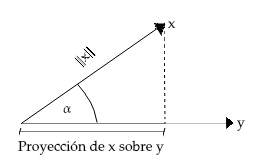
\includegraphics[scale=1]{img/fig001_proyeccion.png} 
\centering
\label{fig:proyeccion}
\end{figure}

Aplicando la igualdad del ángulo entre vectores, y considerando el versor $\breve{y} = \frac{y}{\|y\|}$, resulta:

\begin{equation}
x \cdot y = \|x\| \|y\| \cos(\alpha) \Longrightarrow x \cdot \breve{y} = \|x\| \underbrace{ \cancel{ \| \breve{y} \| } }_{\text{Norma 1}} \cos(\alpha) = \|x\| \cos(\alpha)
\end{equation}

Geométricamente, como se observa en la figura \ref{fig:proyeccion}, la proyección de x sobre y se obtiene como el siguiente vector:

\begin{equation}
\overline{P}_{y}(x) =  \underbrace{ \|x\| \cos(\alpha) }_{\text{Escalar}}  \underbrace{ \breve{y} }_{\text{Versor}}
\end{equation}

\end{document} 